\chapter{Introduction}
\chapterquote{The right question is intellectually superior to finding the right answer.}{Edward O. Wilson}

% Planning
Our ability to make informed decisions depends on how well we can reason about the environment and understand the consequences of our actions.
When decisions involve high-dimensional information or complex dynamics, we increasingly rely on computational tools to augment our understanding or automate this reasoning entirely by using faster measurements, higher fidelity environment models, or more accurate predictions.
Predictive models trained to perform classification or regression play an important role in decision making systems that must act based on partial or high-dimensional information.
Machine learning models are often used in the context of single-step decisions, as it has been shown that they can learn patterns from unstructured or noisy data \cite{murphy2012machine,bishop2006pattern}.
While single-step decisions may be useful in settings such as recommendation systems \cite{covington2016deep} or content moderation \cite{wulczyn2017ex}, many complex real-world problems require making a \textit{sequence} of decisions over time, where each action affects the immediate outcome and shapes future decisions---indicating the necessity to reason for both short-term utility and long-term consequences.


% Sequential planning
Sequential decision making, i.e., \textit{planning}, involves reasoning about actions over time to achieve long-term objectives \cite{dmbook}.
The dependency on long time horizons introduces complexity to the decision making problem.
Long-horizon problems---such as robotic exploration \cite{balaban2020health}, autonomous driving \cite{huang2018hybrid}, and geological drilling operations \cite{mern2023intelligent}---require
\begin{wrapfigure}{r}{0.39\textwidth}
    \begin{center}
        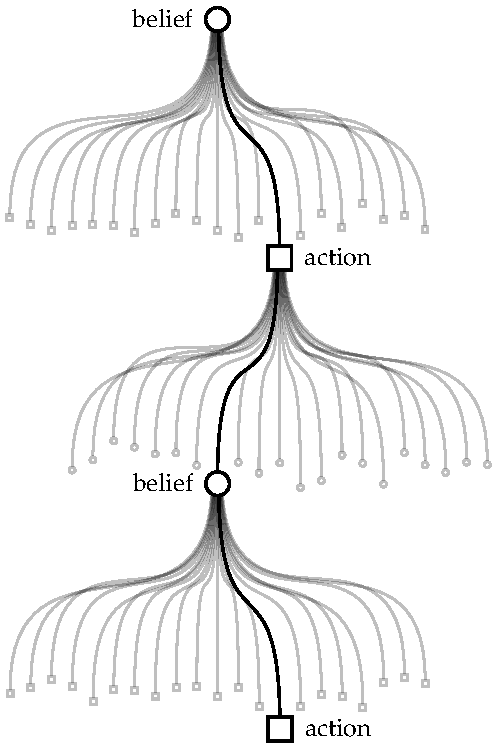
\includegraphics[width=\linewidth]{diagrams/introduction/sequential-search-tree.pdf}
    \end{center}
    \vspace*{-4mm}
    \caption{Sequential search tree (inspired by \textcite{alphago2017movie}).}
    \label{fig:sequential_search_tree}
    \vspace*{-2mm}
\end{wrapfigure}
search-based algorithms \cite{coulom2007efficient} (\cref{fig:sequential_search_tree}) or dynamic programming \cite{bellman1957dynamic} to effectively reason about potential future outcomes.
In these settings, the planning process must operate over a large or continuous set of actions, where enumerating all possibilities is computationally infeasible.
Moreover, real-world problems often have high-dimensional state spaces that describe their environments.
This combined complexity motivates the need for planning algorithms that can scale and generalize to large decision spaces.


% Planning under uncertainty
In addition to the challenges of high-dimensional state and action spaces, real-world planning problems need to operate \textit{under uncertainty}---whether due to stochastic system dynamics or noisy observations.
These planning problems are often modeled as \textit{Markov decision processes} (MDPs) to handle uncertainty in state transition dynamics, and \textit{partially observable MDPs} (POMDPs) to handle state uncertainty \cite{dmbook}.
In such problems, the outcome of an action is not deterministic, and only partial information about the current state is available.
For example, in autonomous driving, we cannot directly observe the true $x$-$y$ position of the vehicle.
Instead, we use noisy measurements from sensors such as GPS or camera feeds to localize and form a \textit{belief} about our position---encoding state uncertainty as shown in \cref{fig:beliefs}---and use probabilistic models to capture how beliefs change over time.
Without modeling belief dynamics, planning algorithms cannot reliably assess risk to ensure safe behavior.


% Safe planning under uncertainty
Real-world problems often require balancing expected performance with the need to maintain safety.
\textit{Safe planning under uncertainty} refers to the design of policies that not only account for uncertainties, but also avoid catastrophic failures.
For example, aircraft collision avoidance systems \cite{kochenderfer2012next} must balance operational suitability by minimizing guidance alerts given to pilots, while also maximizing safety by attempting to avoid midair collisions. 
Therefore, safe planning algorithms require reasoning about the full distribution of possible outcomes and identifying actions that achieve objectives while also satisfying safety constraints.
Incorporating such constraints often requires defining risk bounds, constraining policies to stay within a target level of safety, or model approximations that reduce the dimensionality of the problem to make it tractable.


\begin{figure}[t!]
    \captionsetup{font={small}}
    \centering
    \begin{subfigure}[t]{0.30\linewidth}
        \centering
        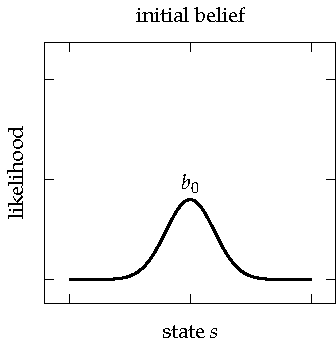
\includegraphics[width=\linewidth]{diagrams/introduction/belief1.pdf}
        \caption{Initial belief at time $t=0$.}
        \label{fig:belief1}
    \end{subfigure}
    \hfill
    \begin{subfigure}[t]{0.30\linewidth}
        \centering
        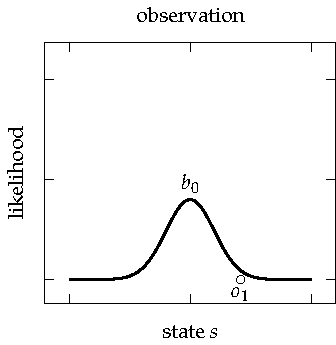
\includegraphics[width=\linewidth]{diagrams/introduction/belief2.pdf}
        \caption{Noisy observation.}
        \label{fig:belief2}
    \end{subfigure}
    \hfill
    \begin{subfigure}[t]{0.30\linewidth}
        \centering
        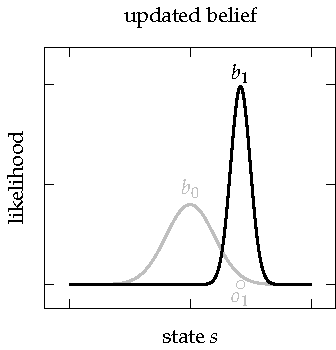
\includegraphics[width=\linewidth]{diagrams/introduction/belief3.pdf}
        \caption{Updated belief at time $t=1$.}
        \label{fig:belief3}
    \end{subfigure}
    \caption{POMDPs encode state uncertainty using \textit{beliefs} (i.e., distributions over states).}
    \label{fig:beliefs}
\end{figure}


% Safe planning planning under uncertainty using surrogate models
While exact safe planning under uncertainty is the goal, it is often computationally intractable in complex, high-dimensional domains.
In practice, simulating all possible outcomes, evaluating risk bounds, or computing belief updates over long horizons can be prohibitively expensive.
To address this limitation, \textit{surrogate models} \cite{forrester2008engineering,goodfellow2016deep} have been increasingly used to approximate costly components of the planning process---such as state-transition dynamics, safety evaluations, or belief updaters---enabling faster and more scalable decision making.
These surrogate models serve as efficient low-dimensional stand-ins for more expensive simulators or domain-specific heuristics.


% Safety validation
Once a policy has been deemed safe through planning to satisfy safety constraints, a crucial next step is to perform \textit{safety validation} \cite{corso2021survey}: validating that the policy behaves safely across the full range of conditions it may encounter during deployment in the real world.
This is particularly important in systems where rare events may exhibit failure modes not seen during planning.
Safety validation has three primary tasks: find failures, find the \textit{most-likely} failure, and estimate the failure probability.
Validating the safety of a policy over a large or continuous operating domain can be computationally expensive, especially when using high-fidelity simulators.
Along with increased planning efficiency, surrogate models offer a benefit during validation by approximating where the system under test may fail---enabling efficient sampling of predicted failures.
Before system deployment, safety validation algorithms can be used as one piece of the full validation process, accelerating the traditional validation loop of simulation and real-world testing.

\paragraph{Research question.}
This thesis attempts to address the challenges of safe planning under uncertainty and safety validation through the use of surrogate models and scalable safety-aware algorithms.
Therefore, our primary research question is the following:
\begin{quote}
    \textit{How can low-dimensional surrogate models be used to enable high-dimensional planning and validation for safety-critical systems?}
\end{quote}

\section{Contributions}
We outline our five main contributions relating to safe planning under uncertainty and efficient safety validation using surrogate models.

\subsubsection{Batched Belief-State Planning}
To scale planning problems to be easily parallelizable, we introduce the \textit{batched planning} problem formulation for MDPs and its extension to POMDPs.
We prove that planning in the batched setting preserves the optimal policy, while also speeding up the lookahead process.

\subsubsection{Inversion Surrogates for Belief Updating}
Methods for parallelized belief updating are required in the batched planning setting.
Therefore, we introduce the \textit{inversion variational autoencoder} ($\mathcal{I}$-VAE), which is a deep conditional generative model that acts as a surrogate to efficiently sample from the posterior belief.
We show that fine-tuning our conditional model to maximize mutual information provides benefits in both planning and estimation.
We demonstrate our approach on a common toy problem of masked hand-written digits using the MNIST dataset \cite{lecun1998gradient} and a novel muon-based intrusion discovery POMDP.
We develop theoretically optimal one-step information-gathering heuristic policies that perform close to optimal in practice.

\subsubsection{Planning and Learning in Belief Space}
To replace hand-crafted heuristics and to generalize POMDP planning algorithms to long-horizon problems, we introduce the \textit{BetaZero} policy iteration algorithm.
We use insights from recent success in game-playing agents \cite{silver2018general} that combine online Monte Carlo tree search (MCTS) planning with learned offline neural network surrogates that replace value function and action selection heuristics.
We address several challenges relating to stochastic belief-state transitions, expensive belief updates given a limit tree search budget, and how to represent non-parametric belief distributions as inputs to the neural network.
We demonstrate the generalizability of our method across various benchmark POMDPs---including robot localization and navigation, robot exploration, and critical mineral exploration---and compare to state-of-the-art online algorithms.
We show that BetaZero scales well given available compute and can learn approximately optimal value functions and action selection policies.
We provide insights into how BetaZero replaces expert heuristics by using learned offline experience to reduce online planning horizons.


\subsubsection{Safe Planning using Failure Surrogates}
As a natural extension to BetaZero for chance-constrained POMDPs, we introduce the \textit{ConstrainedZero} policy iteration algorithm.
In the safety-critical setting, we extend the neural network model to predict the failure probability given a belief.
We then introduce \textit{$\Delta$-MCTS} as a method for safety-aware online planning using the failure probability surrogates to guide the search.
We demonstrate our method on a safety-critical version of robot localization and navigation, an aircraft collision avoidance system, the problem of safe CO$_2$ storage, and an airborne wildfire resource allocation problem.
We show that by separating safety constraints from the primary objective, we can achieve a target level of safety without directly optimizing the balance between rewards and costs. 

\subsubsection{Safety Validation using Probabilistic Surrogates}
We investigate the use of probabilistic surrogate models (i.e., Gaussian processes) for black-box safety validation.
We introduce the \textit{Bayesian safety validation} method that iteratively selects new design points to satisfy the objectives of finding failures, finding likely failures, and ultimately estimating the failure probability over the operating domain of a system.
Our method introduces three new acquisition functions, each with their own safety validation objective.
We demonstrate the method on three test problems, a stochastic POMDP, and a neural network-based runway detection system---treating each system as a black box.
Results from our experiments indicate that Bayesian safety validation finds likely failures (allowing developers to triage appropriately) and can efficiently estimate the failure probability.


\begin{figure}[t]
    \centering
    \resizebox{\linewidth}{!}{
        \begin{tikzpicture}

\tikzset{
    >={Latex[width=2mm,length=2mm]},
    base/.style = {rectangle, rounded corners=1pt, draw=black,
                   minimum width=4.5cm, minimum height=2.25cm,
                   text centered},
    blockstyle/.style = {base, fill=gray!10}
}

%% POMDP loop
\node[blockstyle, rounded corners=25pt, dashed, fill=gray!5, minimum width=20cm, minimum height=6cm] at (0,-0.6) (pomdp) {};

\node[above=10pt of pomdp.south west, anchor=west, xshift=10mm, font=\large] {batched belief-state planning (POMDP)};
\node[below=10pt of pomdp.south west, anchor=west, xshift=10mm, font=\large\color{gray}] {chapter \ref{ch:bbmdp}};


%% Planner
\node[blockstyle] (planner) at (0,0) {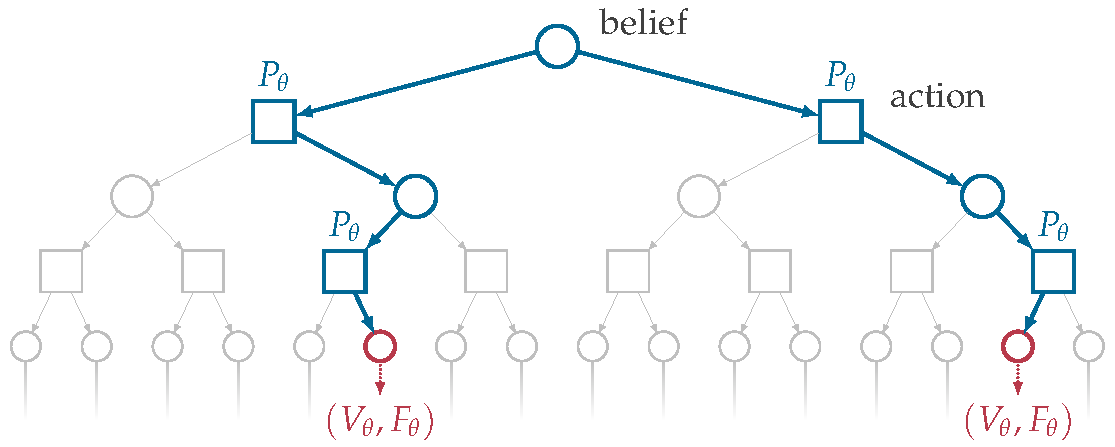
\includegraphics[width=4cm]{diagrams/introduction/tree-search.pdf}};

\node[above=2pt of planner.north, anchor=south, font=\Large] {safe planner};
\node[below=2pt of planner.south, anchor=north, font=\large\color{gray}] {chapters \ref{ch:betazero} and \ref{ch:constrainedzero}};


%% Belief updater
\node[blockstyle, left=2cm of planner] (belief) {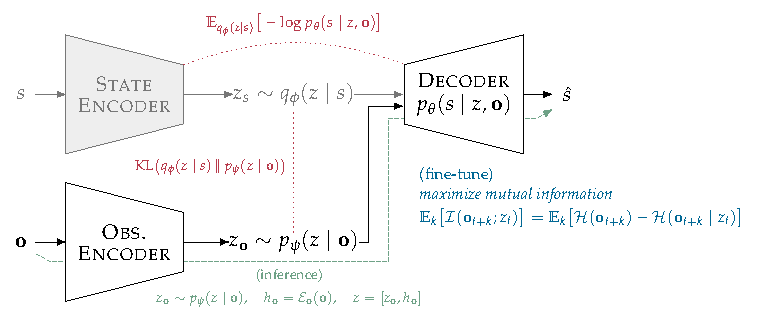
\includegraphics[width=3.75cm]{diagrams/introduction/ivae.pdf}};

\node[above=2pt of belief.north, anchor=south, font=\Large] {belief updater};
\node[below=2pt of belief.south, anchor=north, font=\large\color{gray}] {chapter \ref{ch:ivae}};


%% Environment
\node[blockstyle, right=2cm of planner] (env) {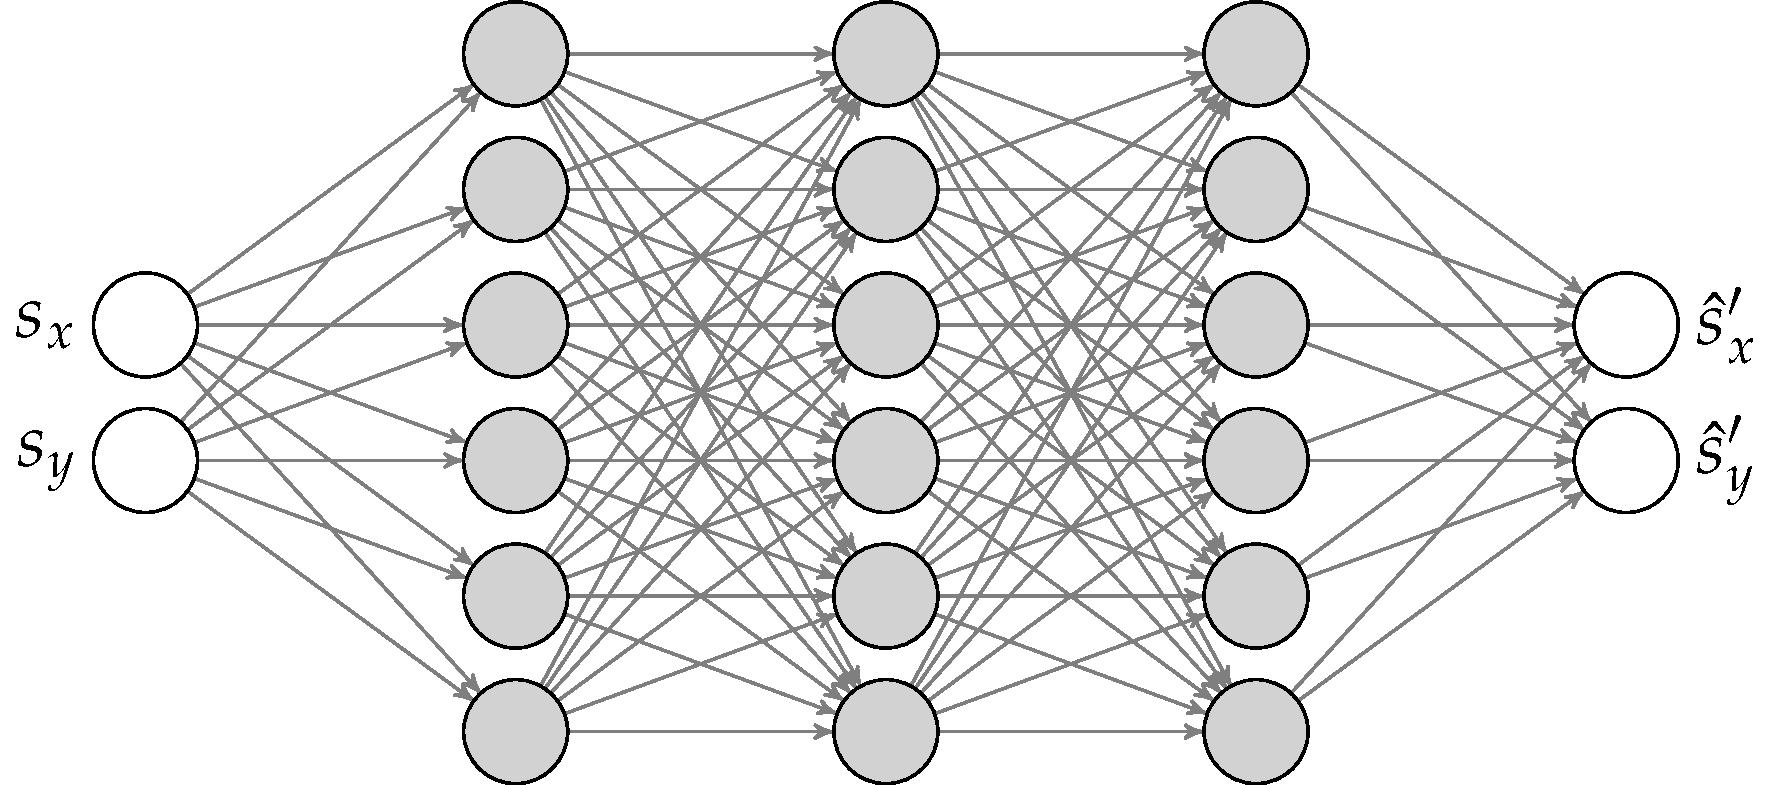
\includegraphics[width=3cm]{diagrams/introduction/env.pdf}};

\node[above=2pt of env.north, anchor=south, font=\Large] {environment};
\node[below=2pt of env.south, anchor=north, font=\large\color{gray}] {chapter \ref{ch:future} (future work)};


%% Bayesian safety validation
\node[blockstyle, rounded corners=25pt, fill=none, minimum width=22cm, minimum height=8cm] at (0,-0.6) (bsv) {};

\node[fill=none, draw=none, anchor=east, font=\large] (input) at ($(bsv.west)+(-7mm,0)$) {\shortstack{adversarial\\input}};
\node[fill=none, draw=none, anchor=west, font=\large] (output) at ($(bsv.east)+(7mm,0)$) {\shortstack{failure\\output}};


%% Arrows
\draw[->, font=\large] (belief) -- (planner) node[midway, above] {belief} node[midway, below] {$b_t$};

\draw[->, font=\large] (planner) -- (env) node[midway, above] {action} node[midway, below] {$a_t$};

\draw[->, font=\large] ($(env.south)-(0,7mm)$) to[out=230, in=310, looseness=0.28] node[midway, above, sloped] {observation} node[midway, below, sloped] {$o_t$} ($(belief.south)-(0,7mm)$);

\draw[->] (input) -- (bsv);
\draw[->] (bsv) -- (output);

\def\offset{6cm}

\draw[->, rounded corners=10pt]
  (output.south)
  -- ++(0,-\offset)
  -- node[blockstyle, midway] (gp) {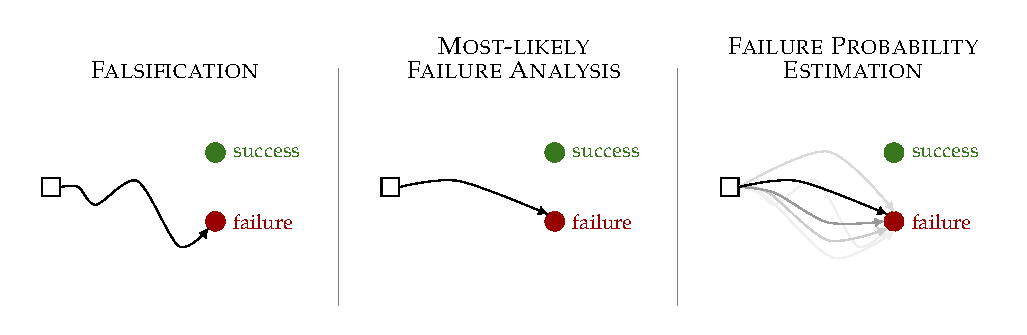
\includegraphics[width=4.5cm]{diagrams/introduction/safety-validation.pdf}} ($(input.south)+(0,-\offset)$)
  -- (input.south);

\node[above=2pt of gp.north, anchor=south, font=\Large] {black-box safety validation};
\node[below=2pt of gp.south, anchor=north, font=\large\color{gray}] {chapter \ref{ch:bsv}};

\end{tikzpicture}
    }
    \caption{Overview of our thesis contributions relating to safe planning and validation.}
    \label{fig:overview}
\end{figure}


\section{Overview}
\Cref{fig:overview} provides an overview of how our contributions are connected in the safe planning and validation process.
The structure of the remaining thesis is organized as follows:

\begin{itemize}
    \item The remainder of \Cref{part:background} provides background on the problems and foundations of the technical methods used in this thesis.
    In \cref{ch:problems}, we provide details about the safety-critical problem domains we study.
    In \cref{ch:preliminaries}, we review technical background on topics including Markov decision processes (MDPs), partially observable MDPs (POMDPs), belief-state MDPs, belief updating methods, offline and online planning algorithms, surrogate modeling, and safety validation.
    \item \Cref{part:planning} explores how to efficiently scale POMDP planning algorithms to high-dimensional problems.
    In \cref{ch:bbmdp}, we introduce the batched planning framework and prove that it preserves the optimal policy.
    In \cref{ch:ivae}, we introduce a surrogate model for belief updating, allowing us to use the batched planning framework efficiently.
    In \cref{ch:betazero}, we introduce a scalable policy iteration algorithm for long-horizon POMDPs that learns from offline experience to reduce online planning horizons.
    \item \Cref{part:safety} explores methods for safe planning at scale and surrogates for safety validation.
    In \cref{ch:constrainedzero}, we introduce a chance-constrained POMDP policy iteration algorithm that learns a failure surrogate through experience to inform safe online planning.
    In \cref{ch:bsv}, we introduce a black-box method to efficiently estimate the failure probability using probabilistic surrogate models.
    \item \Cref{part:conclusions} concludes the thesis and provides future research directions.
    In \cref{ch:summary}, we provide a summary of this thesis.
    In \cref{ch:contributions}, we reiterate the contributions of this thesis, provide explanations for the open-source contributions, and detail our publications.
    Finally, in \cref{ch:future}, we examine the limitations, possible next steps, and extensions to the research provided in this thesis.
\end{itemize}

